\documentclass{article}
\usepackage[utf8]{vietnam}
\usepackage{amsmath}
\usepackage[a4paper, margin=1in]{geometry}
\usepackage[linesnumbered,ruled,vlined]{algorithm2e}
\usepackage{graphicx} % Required for inserting images
\usepackage{tikz} % Required for drawing diagrams
\usepackage{pgf} % Required for tikz

\title{Báo Cáo Tuần 3 Thuật Toán Tách Công Việc Chồng Chéo}


\begin{document}

\maketitle

\section{Mô tả bài toán}
Một nhân viên có thể thực hiện nhiều công việc trong cùng khoảng thời gian. Nếu các công việc của cùng một nhân viên chồng chéo, ta cần tách chúng thành các phân đoạn không chồng chéo để dễ quản lý.Dữ liệu đầu vào gồm danh sách công việc với các thuộc tính:
\begin{itemize}
\item \textbf{Tên công việc} ($T_i$)
\item \textbf{Thời gian bắt đầu} ($T_i^{s}$)
\item \textbf{Thời gian kết thúc} ($T_i^{e}$)
\item \textbf{Người thực hiện} ($T_i^{assignee}$)
\end{itemize}

\section{Mô hình toán học}
Tại một thời điểm $t$, một nhân viên thực hiện các công việc $T_i$ có thời gian:
\begin{equation}
T_i^{d} = T_i^{e} - T_i^{s}
\end{equation}
Nếu có nhiều công việc trùng thời gian của cùng một nhân viên, chúng được chia thành các đoạn không chồng chéo.Tập công việc hoạt động tại thời điểm $t$ được định nghĩa như sau:
\begin{equation}
PS^t = { T_i \mid T_i^{s} \leq t < T_i^{e}, T_i^{assignee} = E }
\end{equation}
Với $E$ là tập hợp các nhân viên.

\section{Thuật toán tách công việc}
\subsection{Mô tả thuật toán}
Thuật toán thực hiện các bước sau:
\begin{enumerate} 
    \item Tạo danh sách các sự kiện gồm thời điểm bắt đầu và kết thúc của từng công việc, kèm theo thông tin nhân viên phụ trách. 
    \item Sắp xếp các sự kiện theo thứ tự thời gian tăng dần. Nếu hai sự kiện xảy ra cùng thời điểm, ưu tiên xử lý sự kiện kết thúc trước sự kiện bắt đầu. 
    \item Duyệt qua các sự kiện theo từng nhân viên: 
    \begin{itemize} \item Theo dõi tập hợp các công việc đang hoạt động tại mỗi khoảng thời gian. 
        \item Khi có sự thay đổi trong tập hợp các công việc (có công việc bắt đầu hoặc kết thúc), ghi nhận một phân đoạn mới. 
        \item Nếu tại một khoảng thời gian có nhiều công việc cùng hoạt động, thuật toán sẽ chia đều khoảng thời gian đó cho các công việc này. 
    \end{itemize}
     \item Trả về danh sách các phân đoạn công việc đã được chia nhỏ và không còn chồng lấn. 
    \end{enumerate}

\section{Mô tả dữ liệu}
\subsection{Danh sách công việc}
\begin{itemize}
    \item \textbf{Tên công việc} ($T_i$): Tên công việc.
    \item \textbf{Thời gian bắt đầu} ($T_i^{s}$): Thời gian bắt đầu công việc.
    \item \textbf{Thời gian kết thúc} ($T_i^{e}$): Thời gian kết thúc công việc.
    \item \textbf{Người thực hiện} ($T_i^{assignee}$): Người thực hiện công việc.
    \item \textbf{Thời gian hoàn thành} ($T_i^{d}$): Thời gian thực hiện công việc.
    \item \textbf{Danh sách phân đoạn} ($T_i^{segments}$): Danh sách các phân đoạn công việc.
    \item \textbf{Thời gian bắt đầu phân đoạn} ($T_i^{segments.s}$): Thời gian bắt đầu phân đoạn.
    \item \textbf{Thời gian kết thúc phân đoạn} ($T_i^{segments.e}$): Thời gian kết thúc phân đoạn.
    \item \textbf{Người thực hiện phân đoạn} ($T_i^{segments.assignee}$): Người thực hiện phân đoạn.
\end{itemize}
\subsection{Mã giả thuật toán}
\begin{algorithm}[H]
    \small
    \SetAlgoLined
    \KwData{Danh sách công việc $\{T_i\}$}
    \KwResult{Danh sách phân đoạn công việc không chồng chéo}
    \SetKwProg{Fn}{Function}{:}{}
    \Fn{splitTasks{$tasks$}}{
        $events \gets \emptyset$\;
        \ForEach{$task \in tasks$}{
            $events.append((task.startTime, 'start', task.name, task.assignee))$\;
            $events.append((task.endTime, 'end', task.name, task.assignee))$\;
        }
        $sort(events \text{ by time ascending, ưu tiên } 'end' \text{ trước } 'start')$\;
        
        $activeTasks \gets \{\}$ \tcp*{Map từ assignee $\to$ tập công việc đang thực hiện}
        $prevTime \gets \{\}$ \tcp*{Map từ assignee $\to$ thời gian trước đó}
        $segmentCounters \gets \{\}$ \tcp*{Map từ assignee $\to$ bộ đếm cho từng task}
        $result \gets \emptyset$\;
        
        \ForEach{$event \in events$}{
            $assignee \gets event.assignee$\;
            \If{$assignee \notin activeTasks$}{
                $activeTasks[assignee] \gets \emptyset$\;
                $prevTime[assignee] \gets null$\;
                $segmentCounters[assignee] \gets \emptyset$\;
            }
            $tasksSet \gets activeTasks[assignee]$\;
            $counters \gets segmentCounters[assignee]$\;
            
            \If{$prevTime[assignee] \neq null \text{ and } tasksSet \neq \emptyset \text{ and } prevTime[assignee] \neq event.time$}{
                $duration \gets event.time - prevTime[assignee]$\;
                $splitDuration \gets duration / tasksSet.size$\;
                $offset \gets 0$\;
                \ForEach{$taskName \in tasksSet$}{
                    $segmentStart \gets prevTime[assignee] + offset$\;
                    $segmentEnd \gets segmentStart + splitDuration$\;
                    \If{$counters[taskName]$ chưa tồn tại}{
                        $counters[taskName] \gets 1$\;
                    }
                    $result.append(Segment(taskName + '.' + counters[taskName], segmentStart, segmentEnd, assignee))$\;
                    $counters[taskName]++$\;
                    $offset \gets offset + splitDuration$\;
                }
            }
            
            \If{$event.type == 'start'$}{
                $tasksSet.add(event.task)$\;
            }
            \Else{
                $tasksSet.remove(event.task)$\;
            }
            
            $prevTime[assignee] \gets event.time$\;
        }
        \KwRet $result$\;
    }
\end{algorithm}

\section{Ví dụ minh họa}
\subsection{Dữ liệu đầu vào}
\begin{center}
    \begin{tabular}{|c|c|c|c|}
        \hline
        Tên công việc & Thời gian bắt đầu & Thời gian kết thúc & Người thực hiện \\
        \hline
         A & 2025-02-12 00:00 & 2025-02-20 00:00 & E1 \\
        \hline
         B & 2025-02-14 00:00 & 2025-02-21 00:00 & E1 \\
        \hline
         C & 2025-02-18 08:00 & 2025-02-20 00:00 & E1 \\
        \hline
         D & 2025-02-16 16:00 & 2025-02-18 08:00 & E2 \\
        \hline
    \end{tabular}
\end{center}
\subsection{Kết quả}
\begin{center}
    \begin{tabular}{|c|c|c|c|}
        \hline
        Tên công việc & Thời gian bắt đầu & Thời gian kết thúc & Người thực hiện \\
        \hline
         A.1 & 2025-02-12 00:00 & 2025-02-14 00:00 & E1 \\
        \hline
         A.2 & 2025-02-14 00:00 & 2025-02-16 00:00 & E1 \\
        \hline
         B.1 & 2025-02-16 00:00 & 2025-02-18 00:00 & E1 \\
        \hline
         D.1 & 2025-02-16 16:00 & 2025-02-18 08:00 & E2 \\
        \hline
         A.3 & 2025-02-18 00:00 & 2025-02-18 16:00 & E1 \\
        \hline
         B.2 & 2025-02-18 16:00 & 2025-02-19 08:00 & E1 \\
        \hline
         C.1 & 2025-02-19 08:00 & 2025-02-20 00:00 & E1 \\
        \hline
         B.3 & 2025-02-20 00:00 & 2025-02-21 00:00 & E1 \\
        \hline
    \end{tabular}
\end{center}

    Chú thích: A.1, A.2, A.3 là phân đoạn của công việc A, B.1, B.2, B.3 là phân đoạn của công việc B, C.1 là phân đoạn của công việc C.
\subsection{Demo}
Trước khi phân đoạn:
\begin{center}
    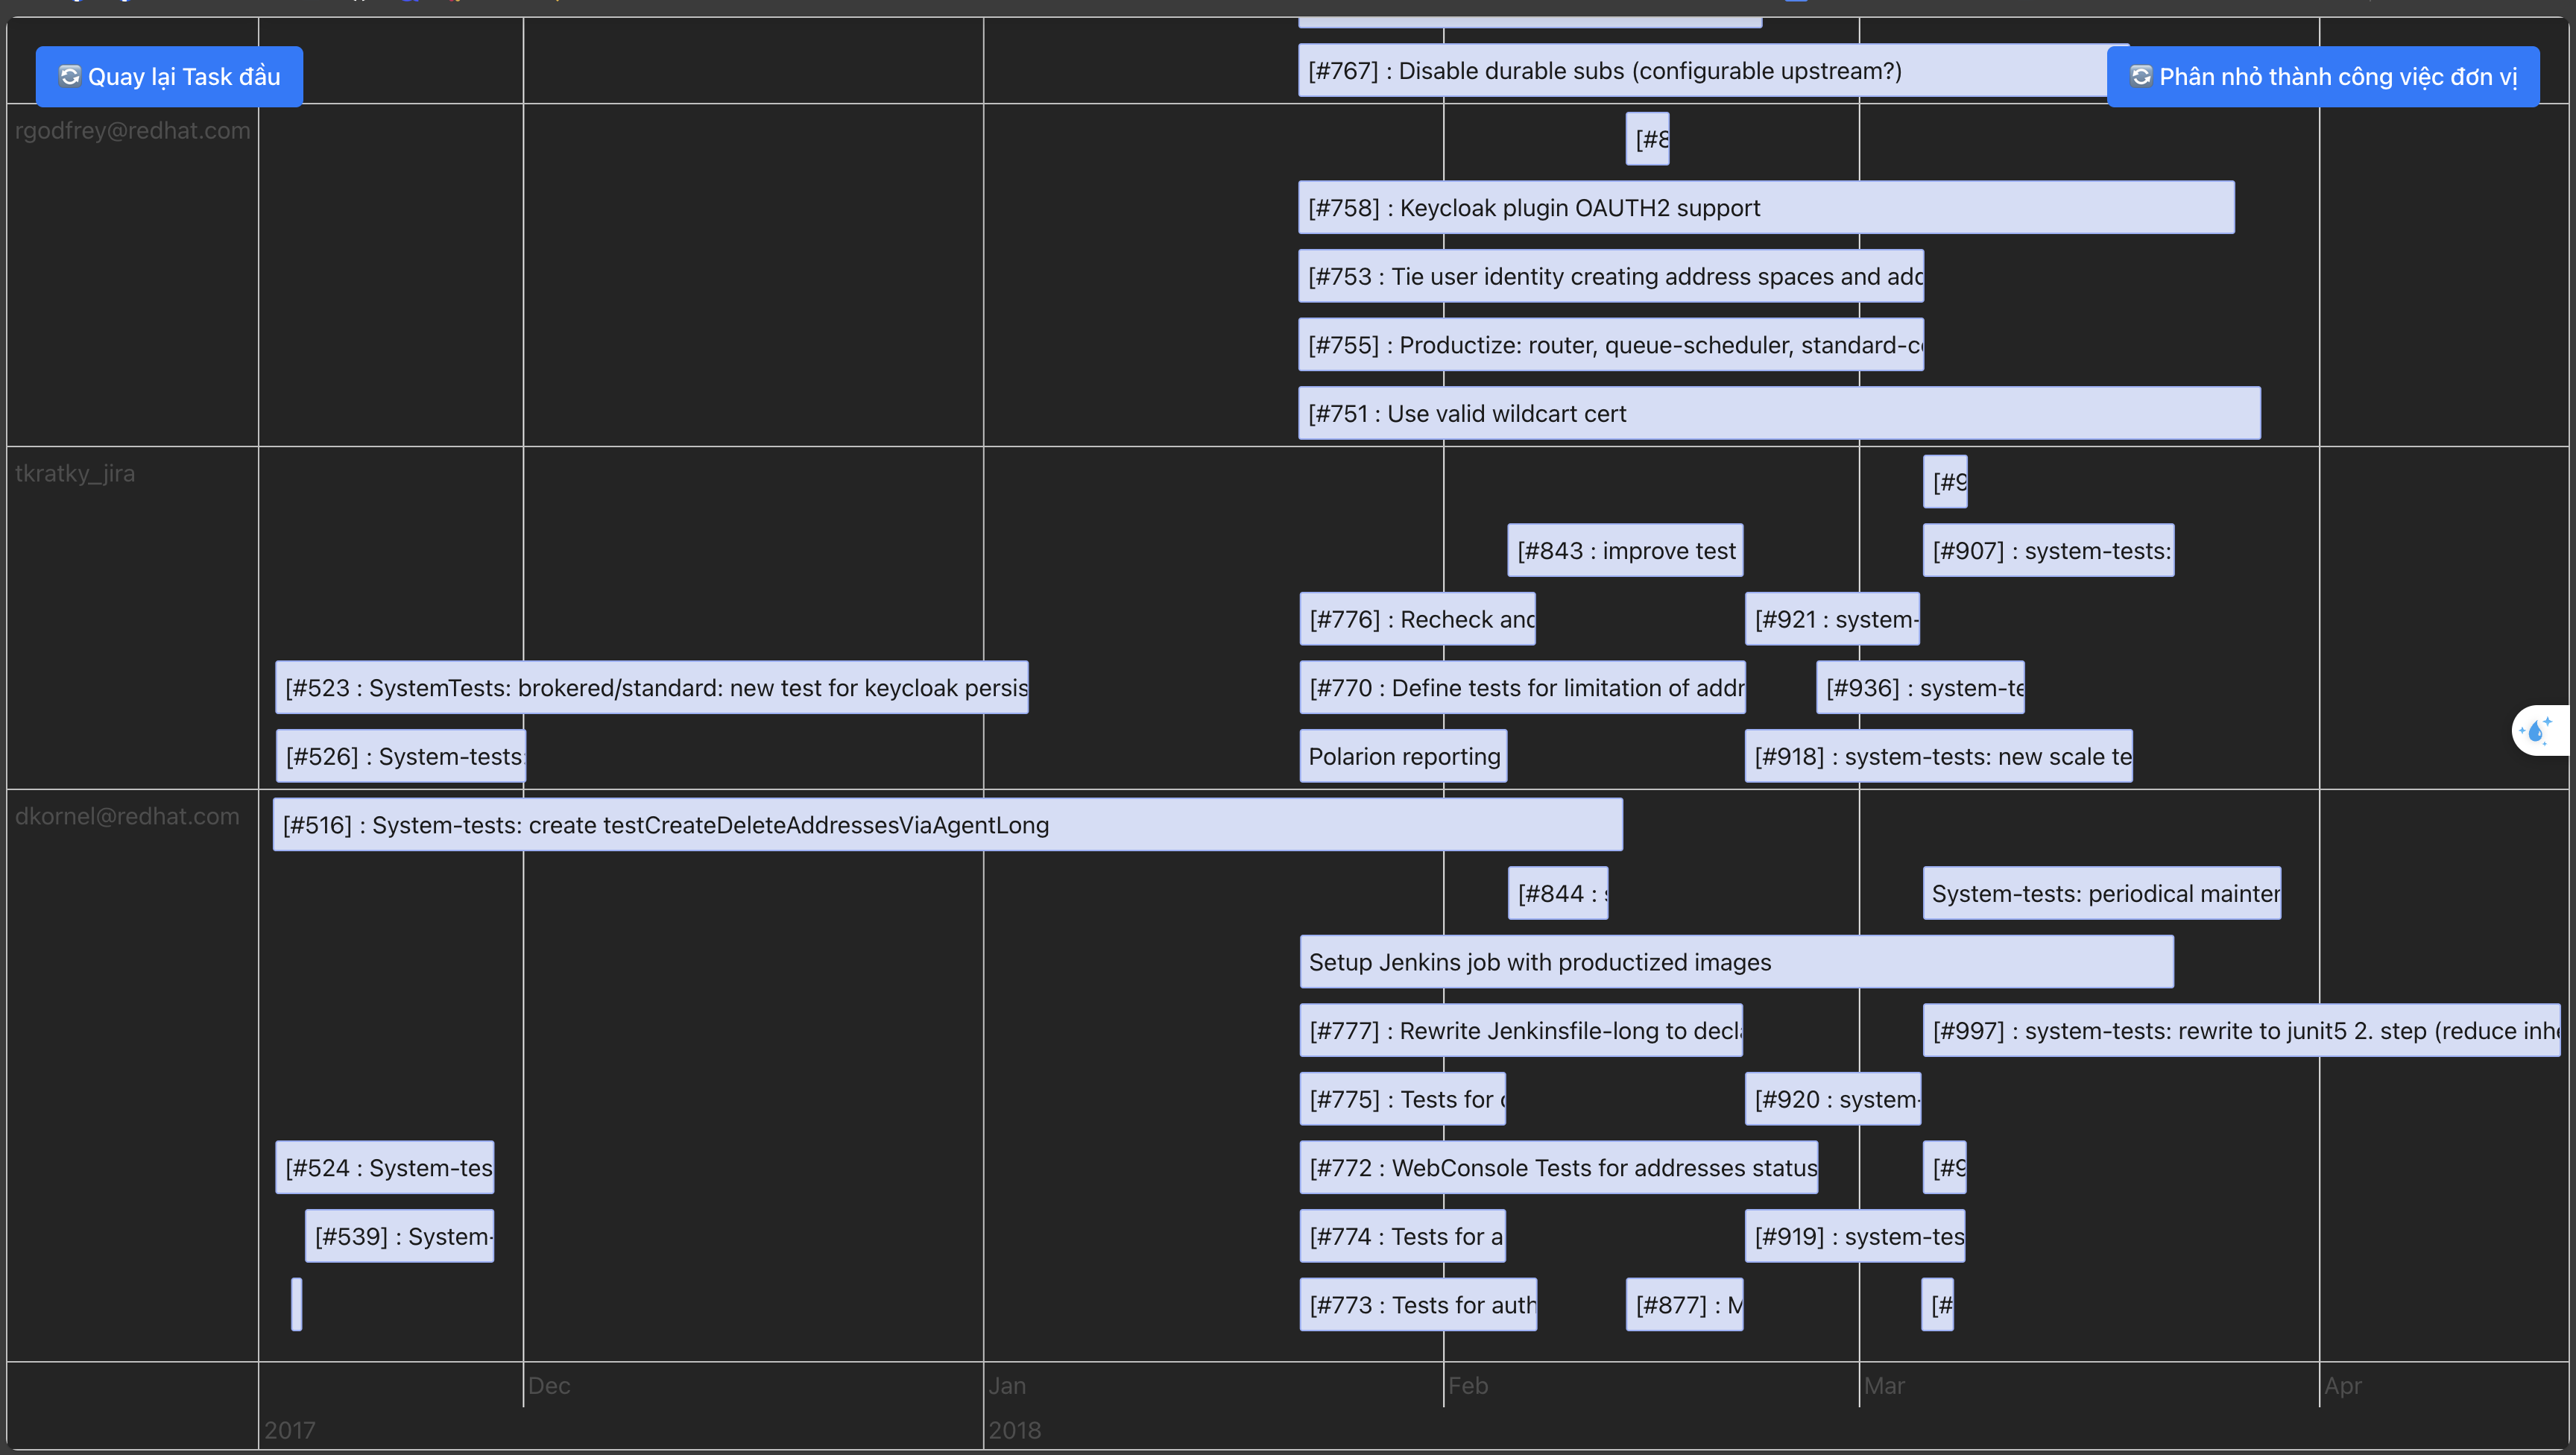
\includegraphics[width=0.8\textwidth]{W3/demo.png}
\end{center}
Sau khi phân đoạn:
\begin{center}
    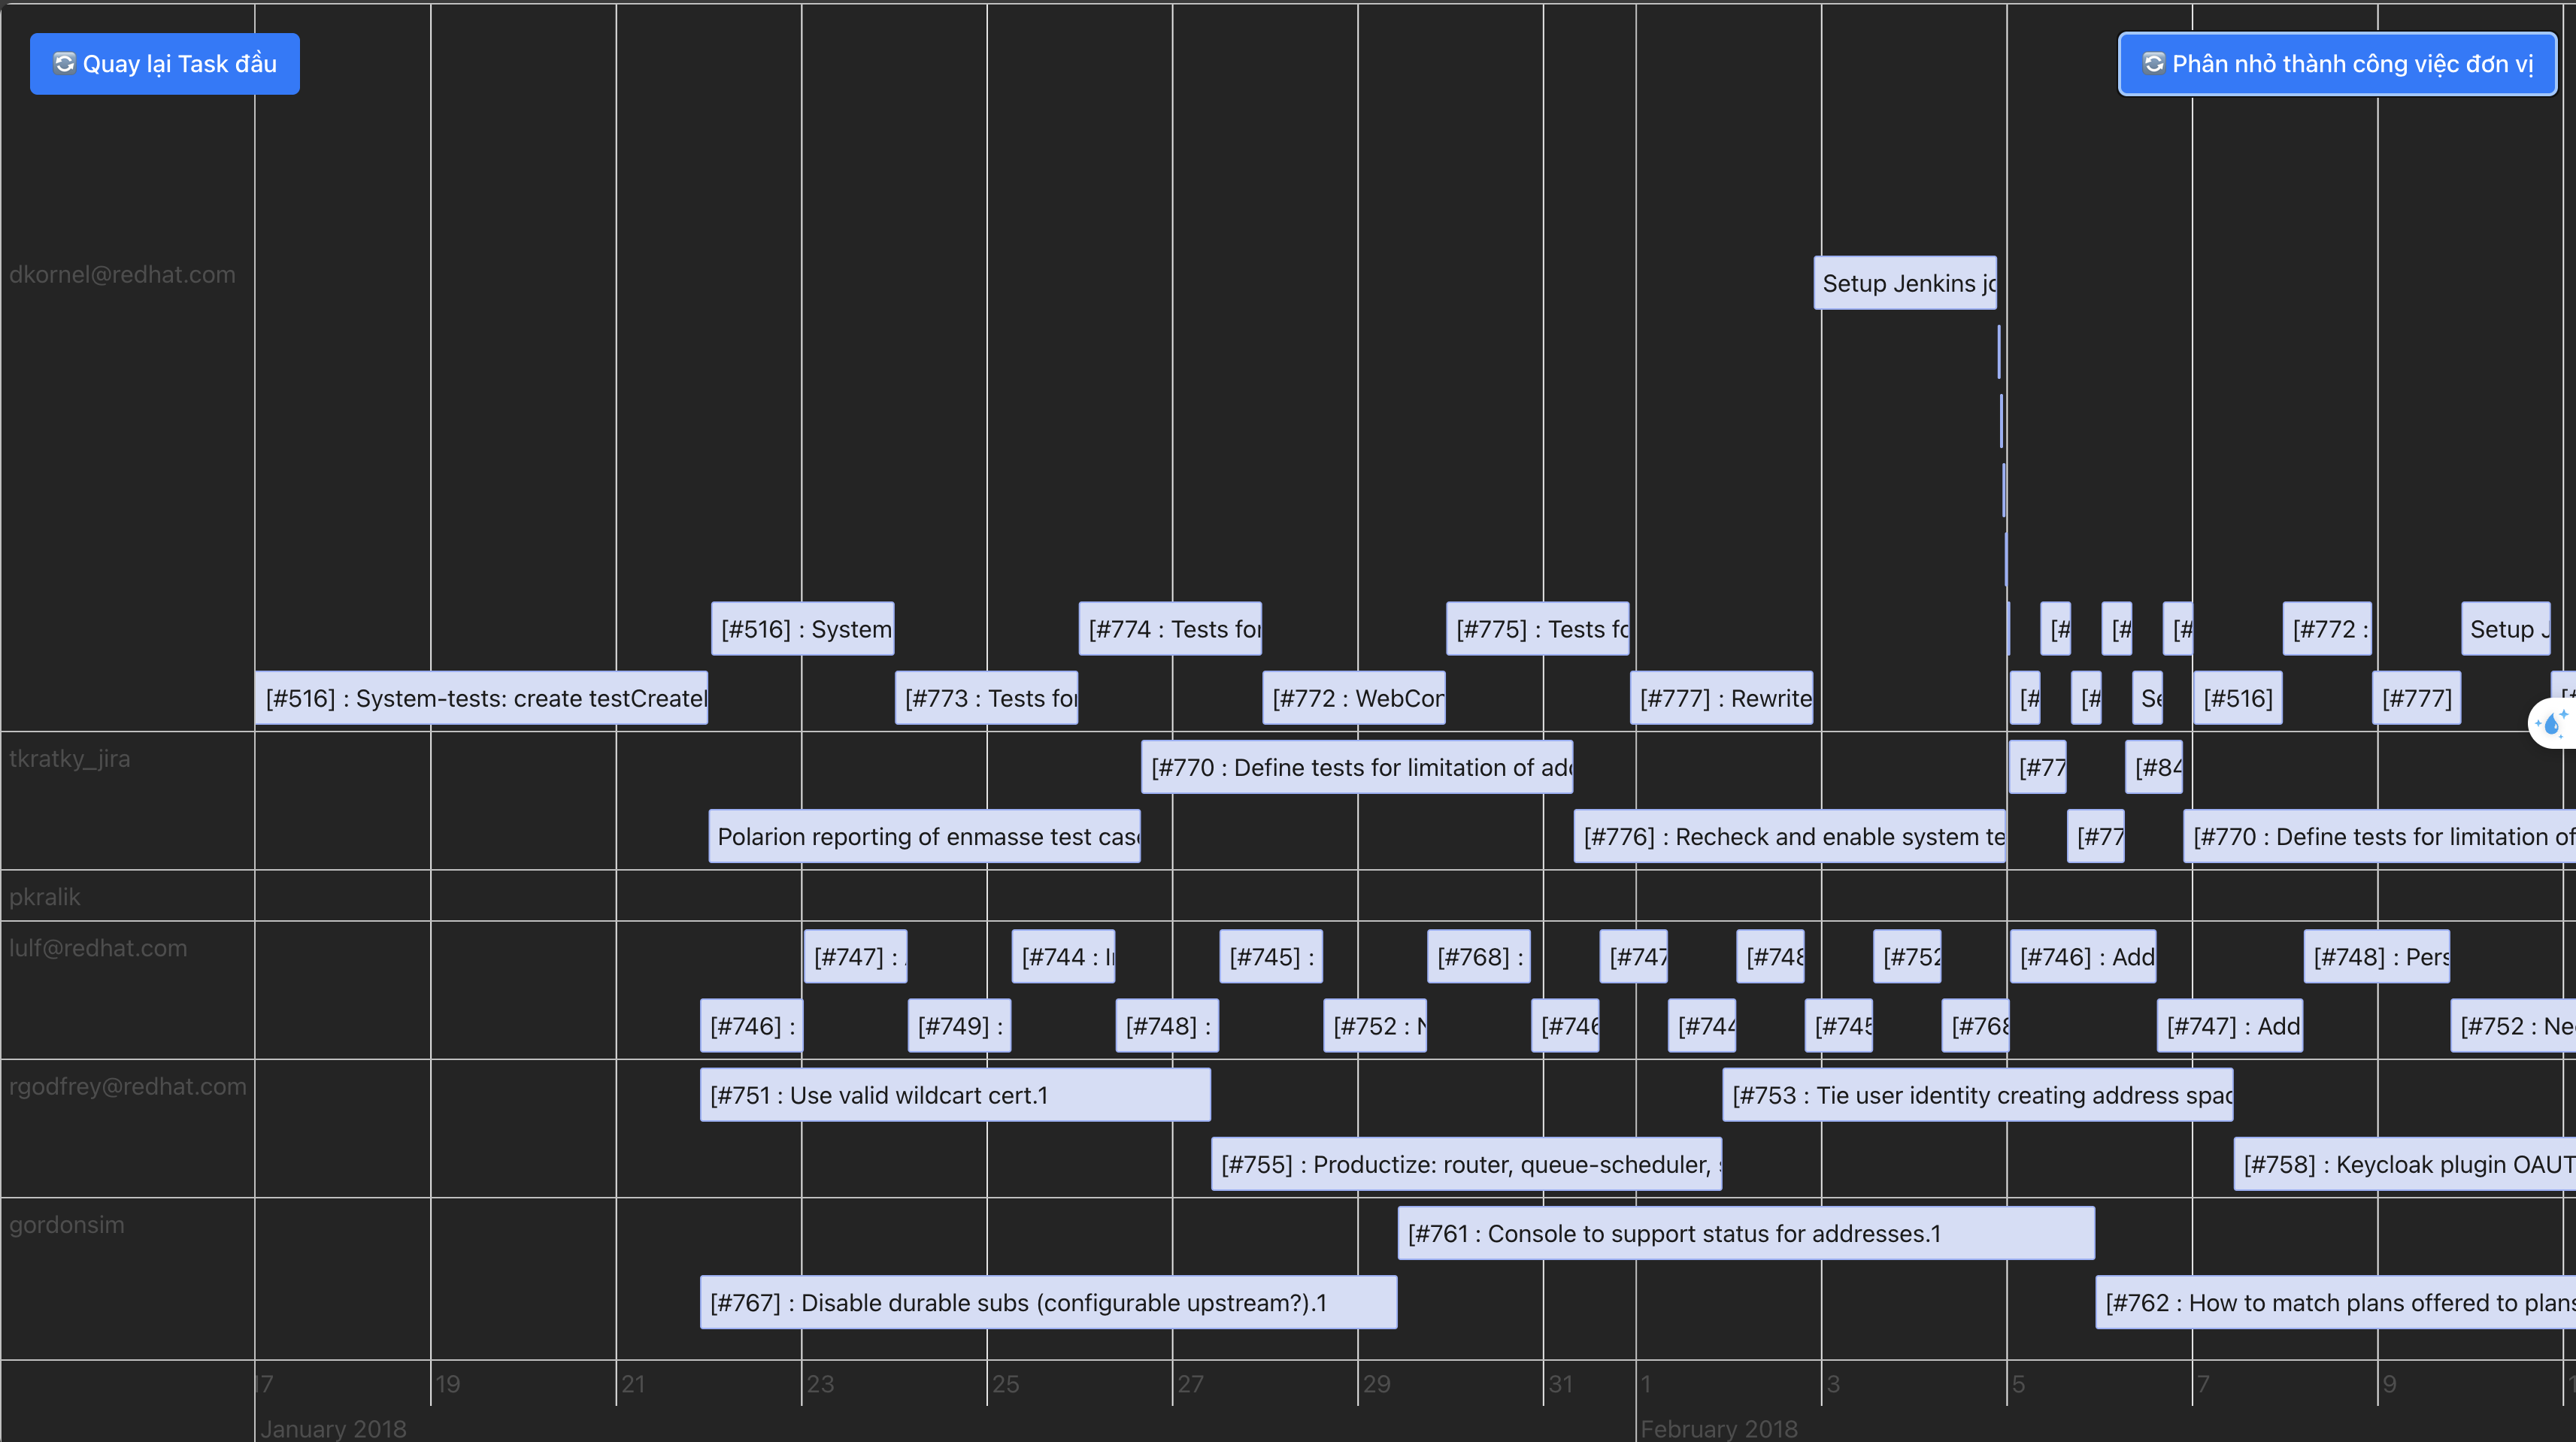
\includegraphics[width=0.8\textwidth]{W3/demo2.png}
\end{center}
\section{Kết luận}
Thuật toán giúp chia nhỏ công việc chồng chéo theo nhân viên, đảm bảo không có thời gian nào bị trùng lặp giữa các công việc của cùng một người. Điều này giúp quản lý công việc dễ dàng và trực quan hơn.
\end{document}